\chapter{Results}

In this project, we have total of seven metrics that we wanted to classify using machine learning model. The results are analysed for individual metrics.

\section{Classification of ALUTS}
\begin{figure}[h!]
\centering
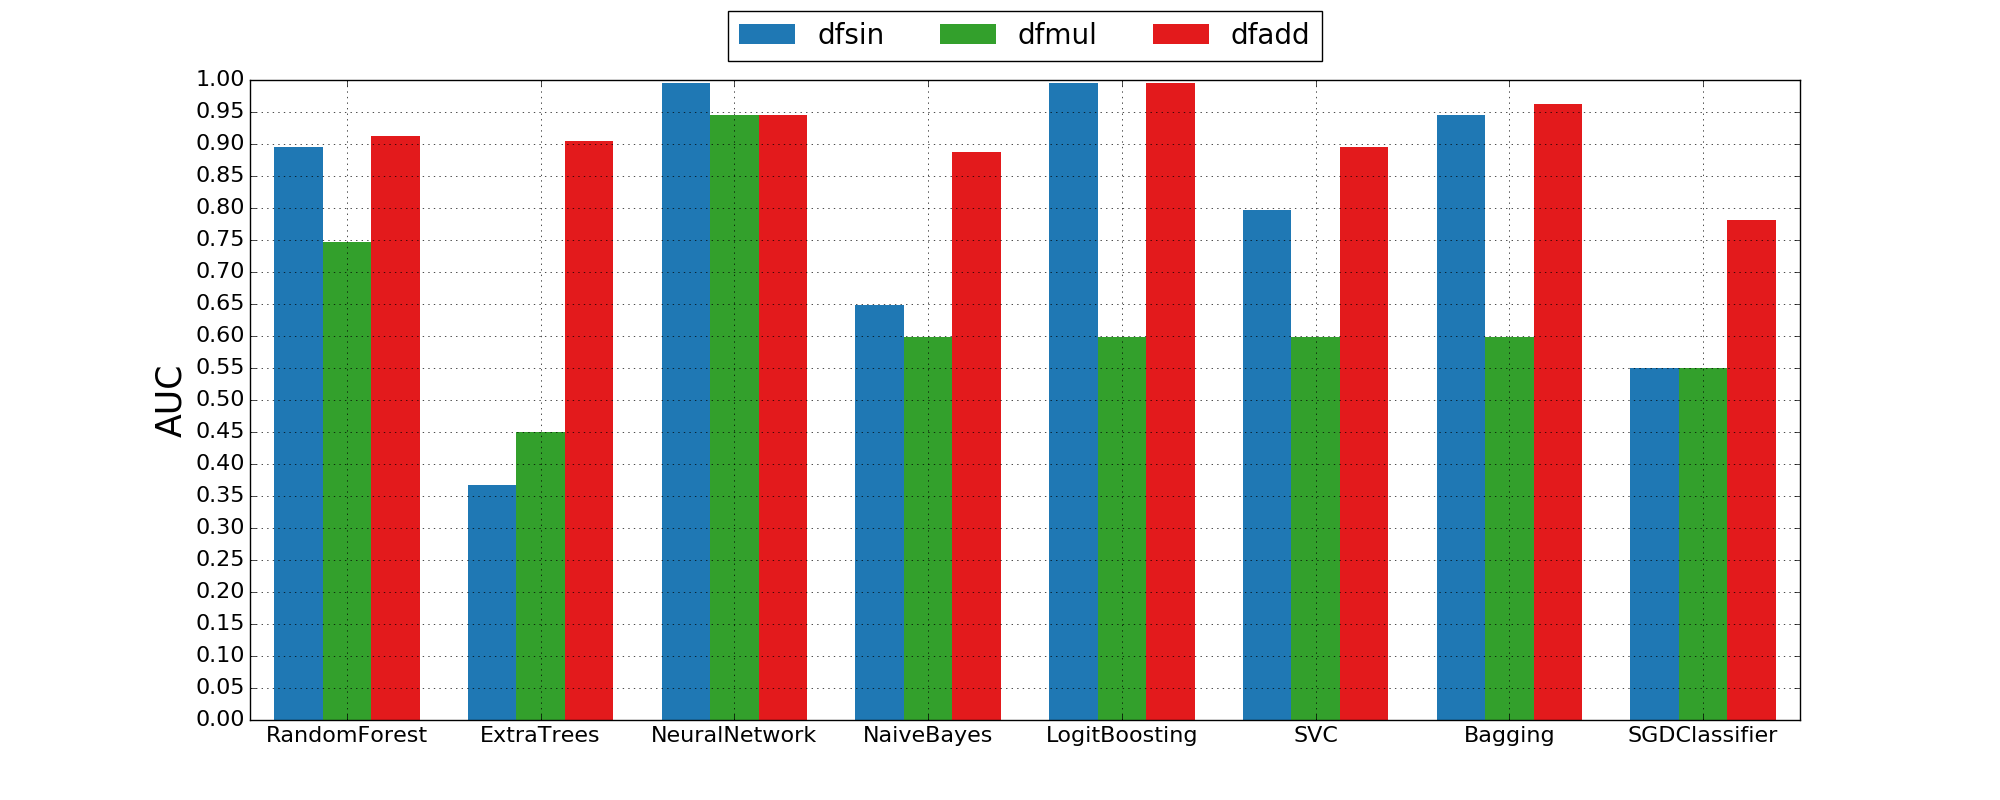
\includegraphics[scale=0.3]{ALUTs_auc_plot.png}
\caption{AUC bar chart for ALUTs}
\label{figure:ALUTs_auc_plot}
\end{figure}

Figure \ref{figure:ALUTs_auc_plot} showed the AUC score for all algorithms that are used to classify ALUTs. Performance variations can be seen clearly. NeuralNetwork classifier has the highest average AUC score of 0.963. ExtraTrees achieved the average AUC score of 0.57 which is the lowest among the eight classifiers and it is followed by SGDClassifier. The reason why SGDClassifier performed poorly is because the data are not linearly separable. Most impressive fact is that RandomForest performed better than ExtraTrees even though ExtraTrees is expected to perform better due to its true more randomness. This happened due to the fact that the data sets and the number of features are relatively small. With the increase of data sets, ExtraTrees should perform better than RandomForest.

\section{Classification of Kernel Fmax}

\begin{figure}[h!]
\centering
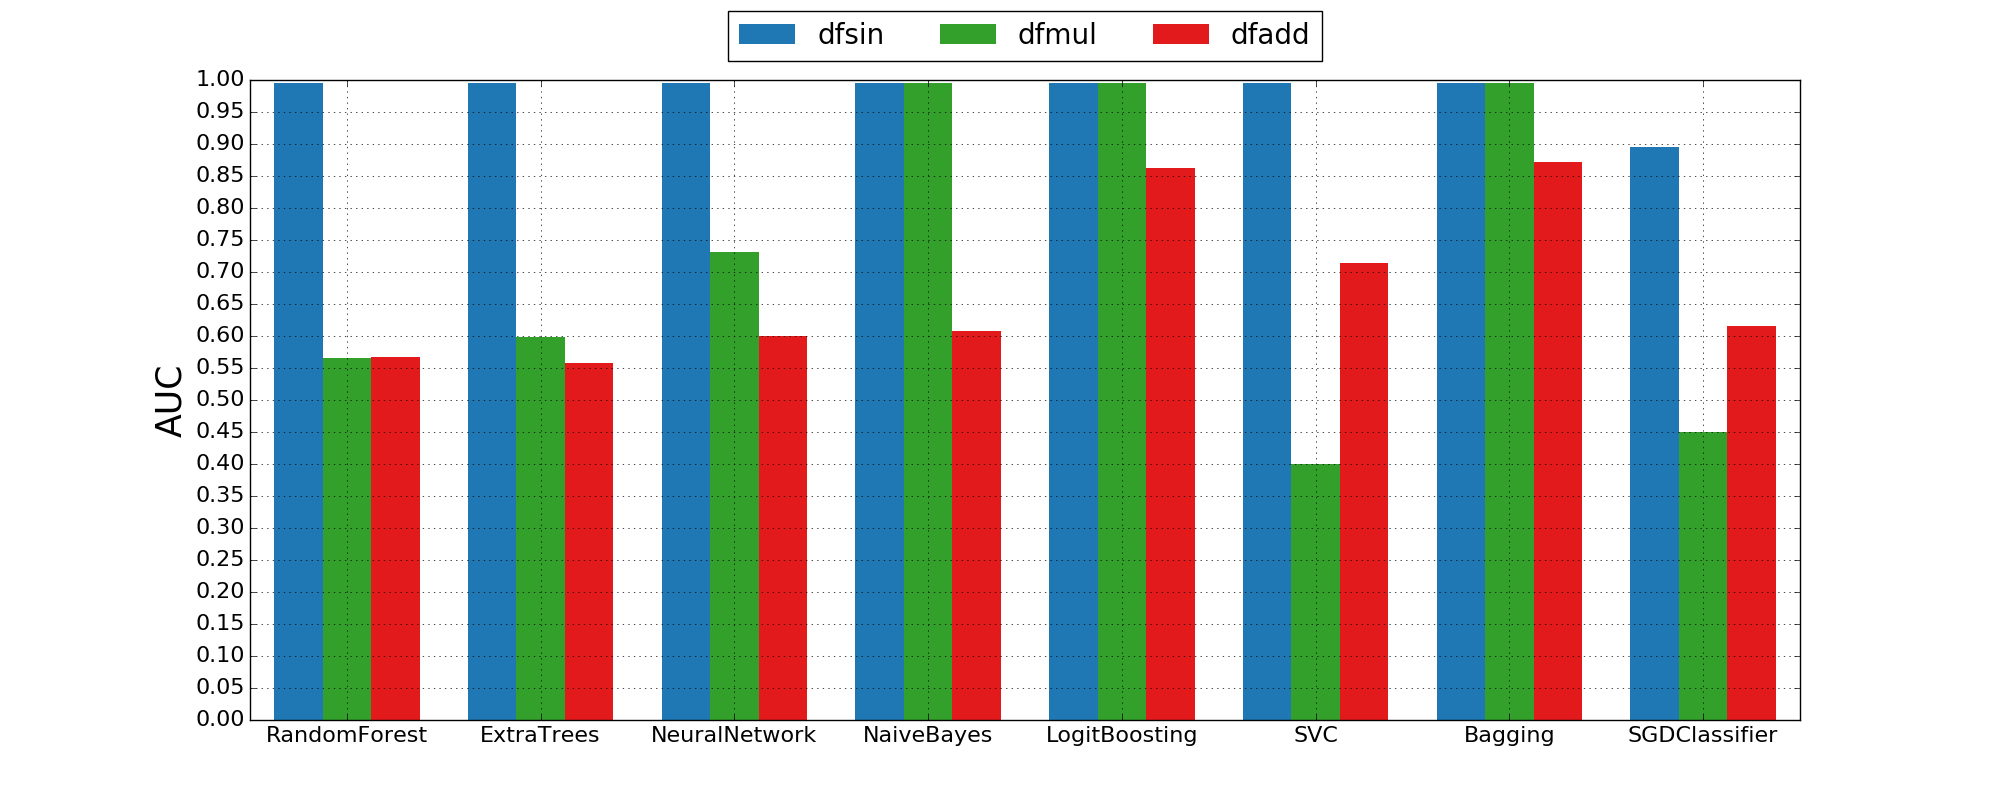
\includegraphics[scale=0.3]{KernelFmax_auc_plot.png}
\caption{AUC bar chart for Kernel Fmax}
\label{figure:kernelfmax_auc_plot}
\end{figure}

\section{Classification of Logic Utilization}

\begin{figure}[h!]
\centering
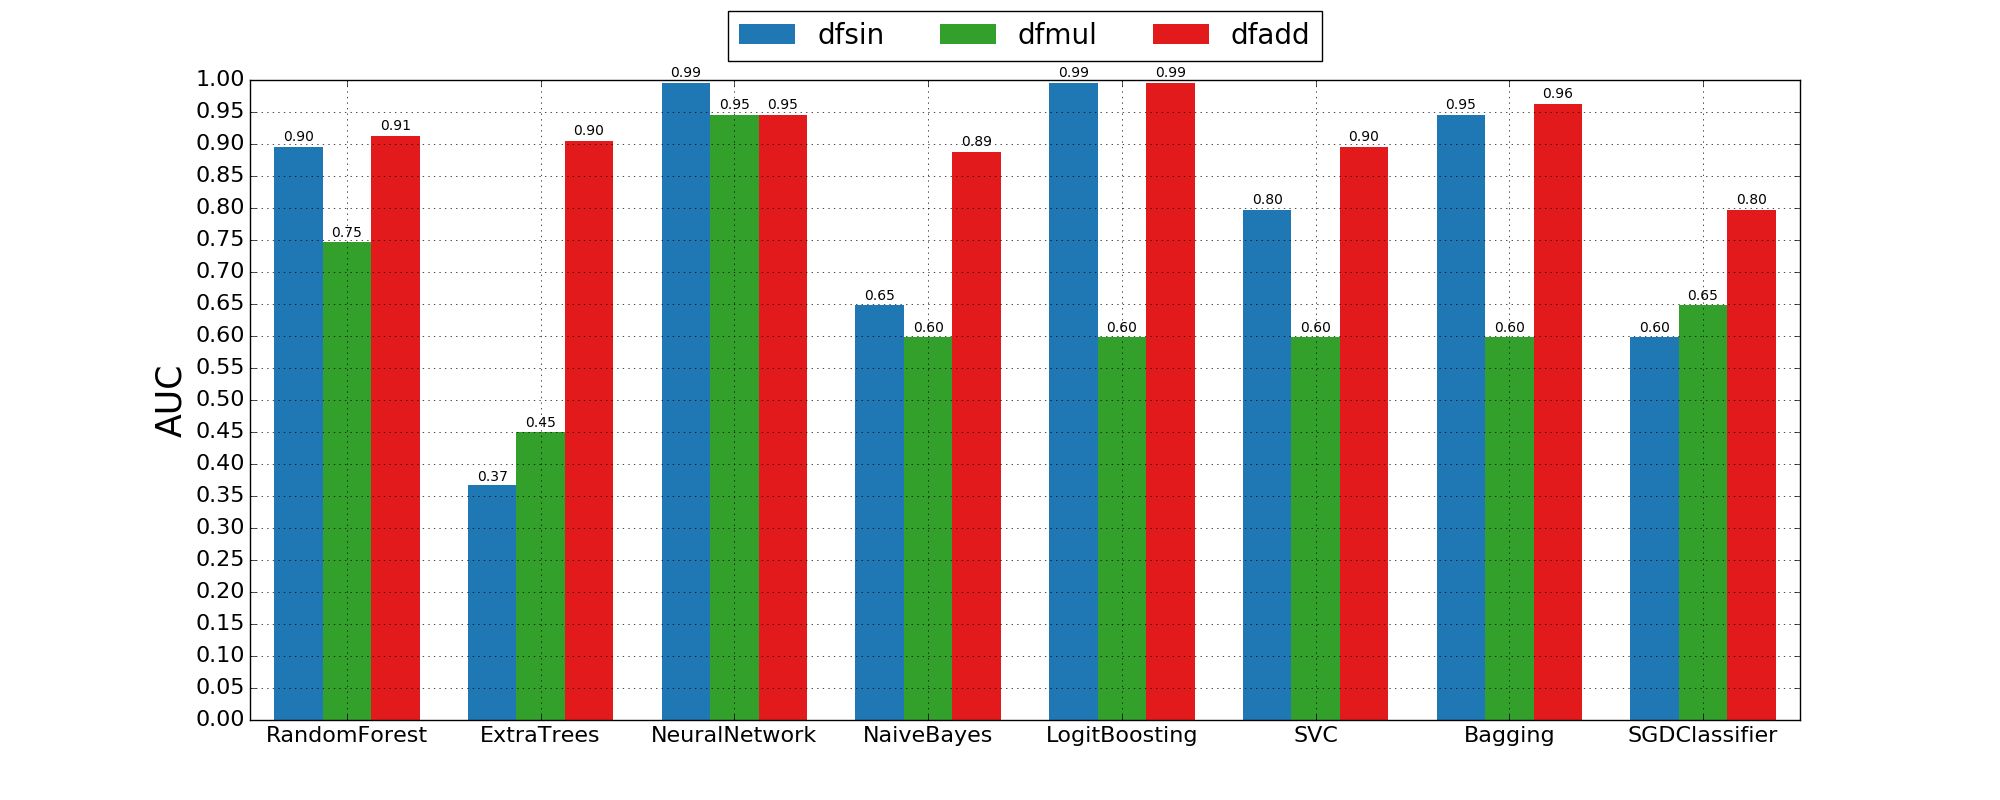
\includegraphics[scale=0.3]{LogicUtilization_auc_plot.png}
\caption{AUC bar chart for Logic Utilization}
\label{figure:LogicUtilization_auc_plot}
\end{figure}

\section{Classification of RAM Blocks}

\begin{figure}[h!]
\centering
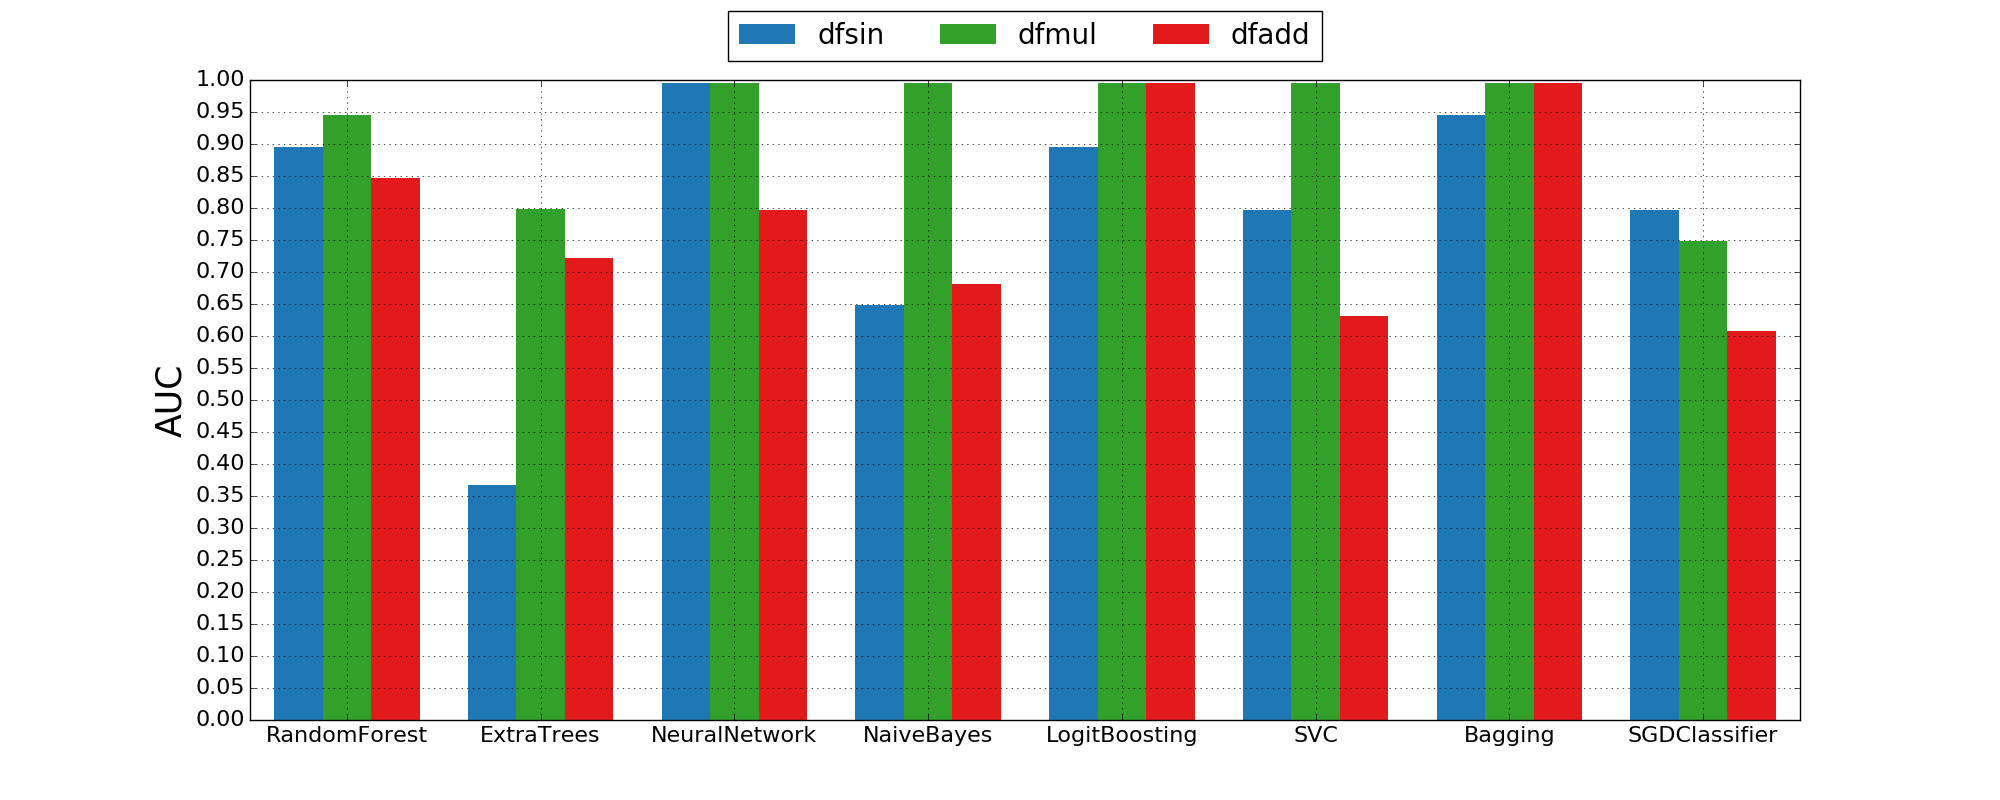
\includegraphics[scale=0.3]{RAMBlocks_auc_plot.png}
\caption{AUC bar chart for RAM Blocks}
\label{figure:RAMBlocks_auc_plot}
\end{figure}

\section{Classification of DSP Blocks}

For DSP Blocks data, there are no variation of data in dfadd benchmark data as they all have the value of zero.

\begin{figure}[h!]
\centering
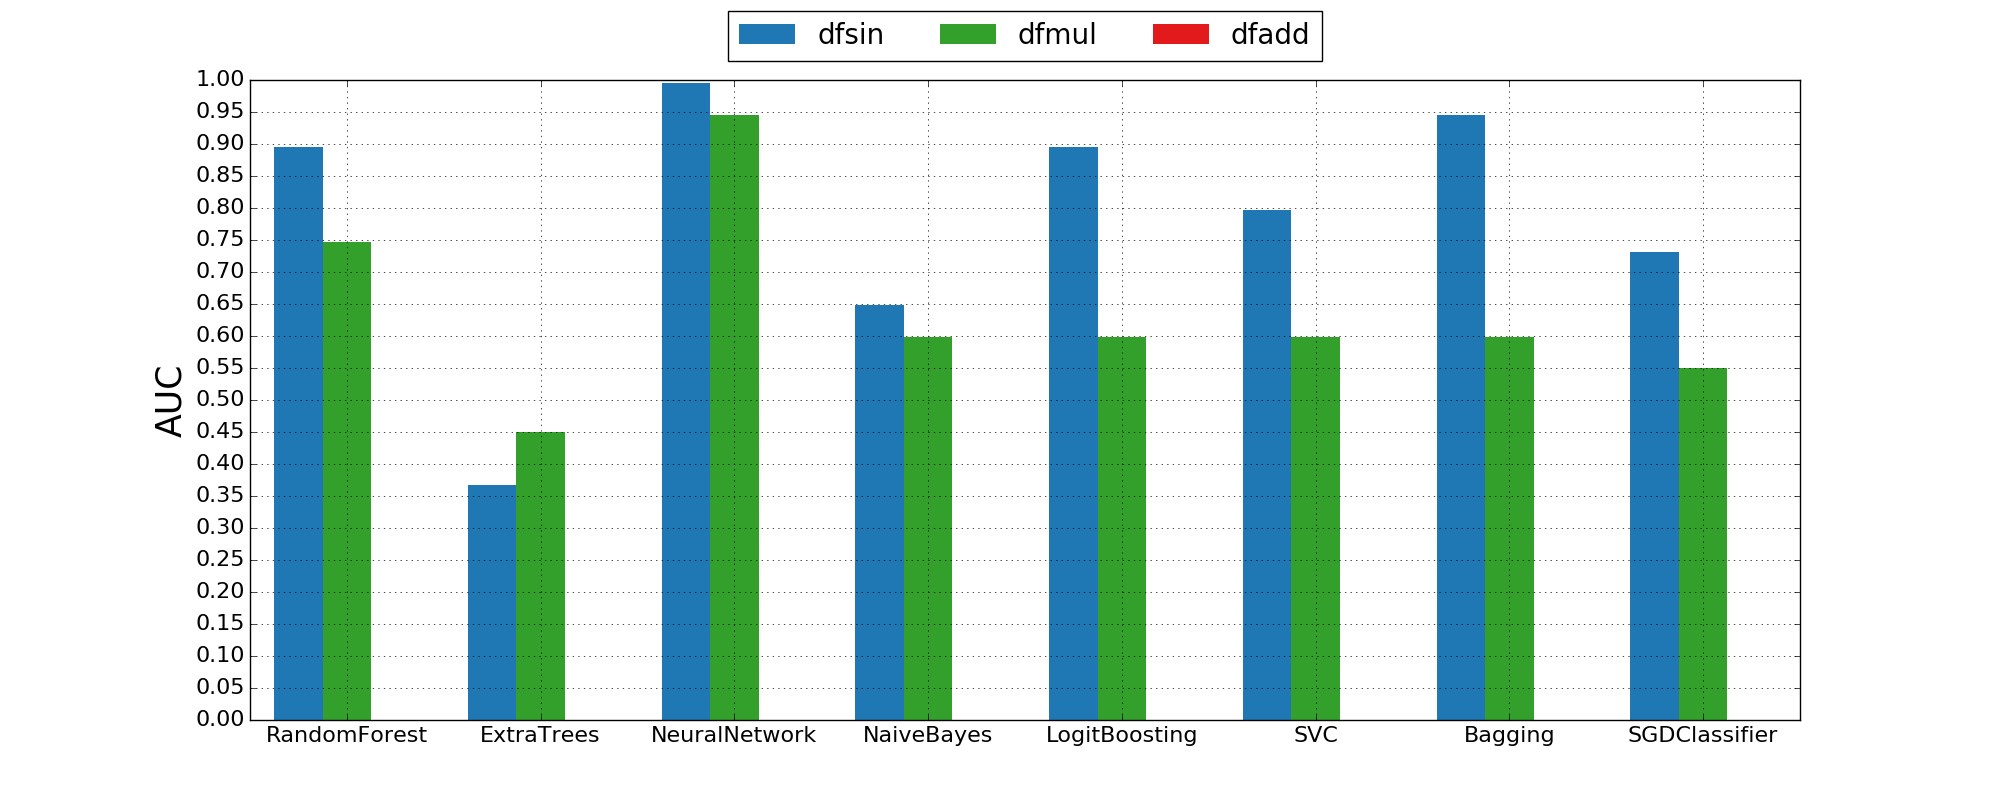
\includegraphics[scale=0.3]{DSPBlocks_auc_plot.png}
\caption{AUC bar chart for DSP Blocks}
\label{figure:dsp_auc_plot}
\end{figure}

Figure \ref{figure:dsp_auc_plot} showed the AUC score for all algorithms that are used to classify DSP blocks. The classification performance of all algorithms for DSP Blocks have the similar analogy as the ALUTs classification with NeuralNetwork being the top classifiers among the eight.

\section{Classification of Memory Bits}
\begin{figure}[h!]
\centering
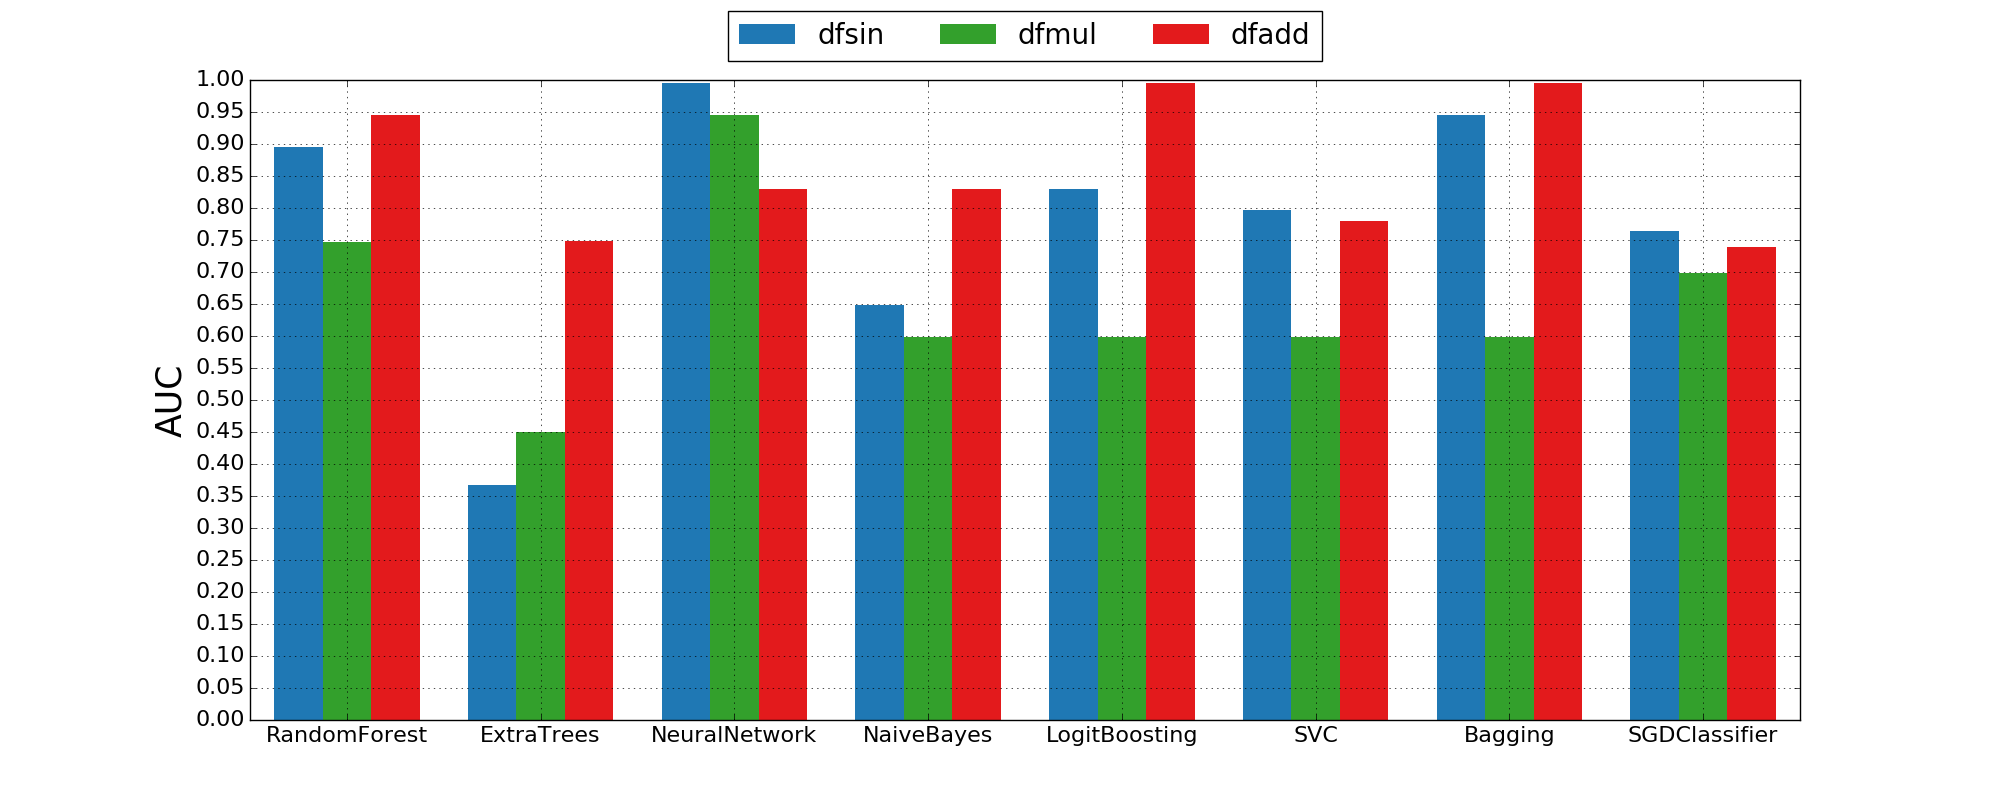
\includegraphics[scale=0.3]{MemoryBits_auc_plot.png}
\caption{AUC bar chart for Memory Bits}
\label{figure:MemoryBits_auc_plot}
\end{figure}

\section{Classification of Registers}
\begin{figure}[h!]
\centering
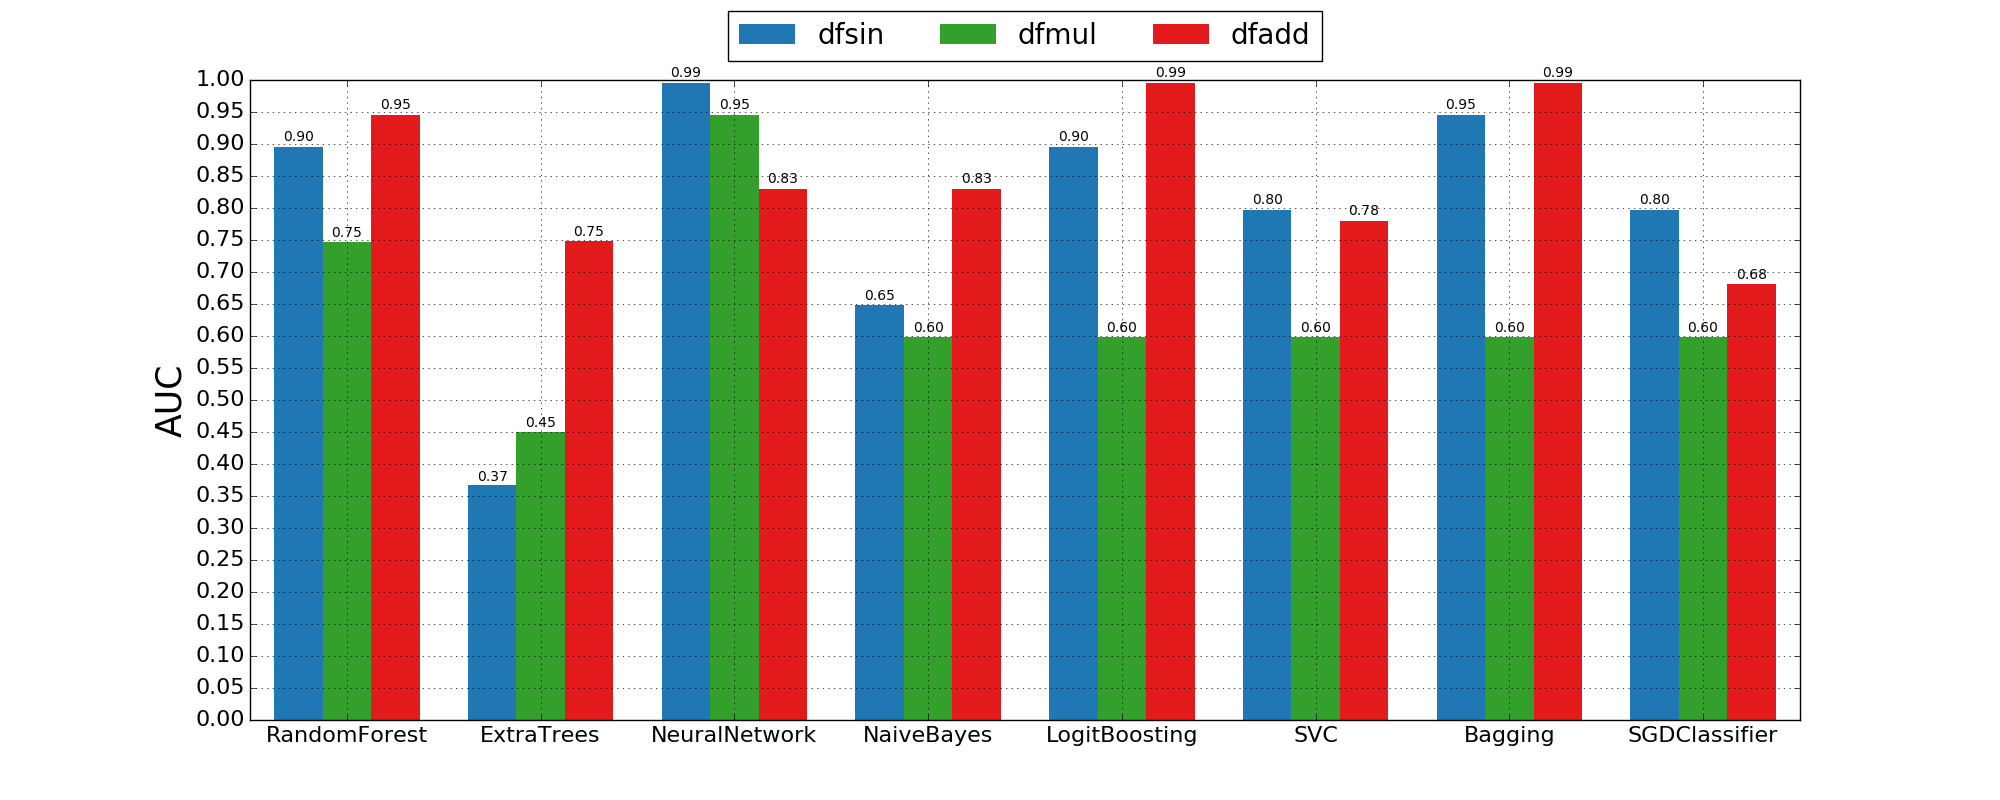
\includegraphics[scale=0.3]{Registers_auc_plot.png}
\caption{AUC bar chart for Registers}
\label{figure:Registers_auc_plot}
\end{figure}

\begin{figure}[h!]
\centering
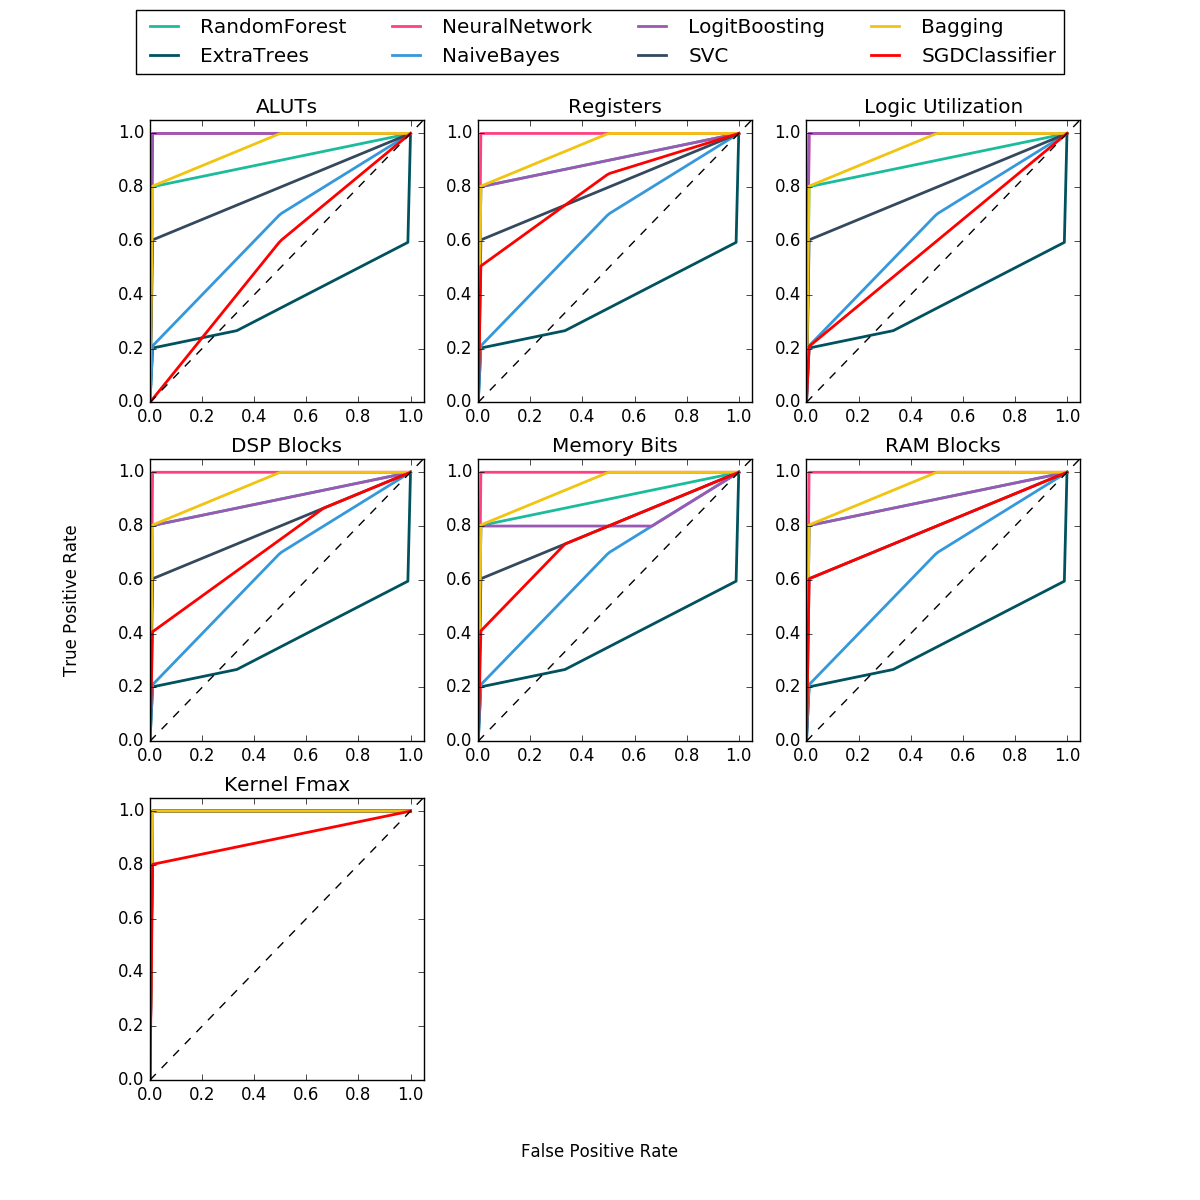
\includegraphics[scale=0.4]{dfsin_roc_curve.png}
\caption{ROC curve for dfsin benchmarks}
\label{figure:dfsin_roc_curve}
\end{figure}

\begin{figure}[h!]
\centering
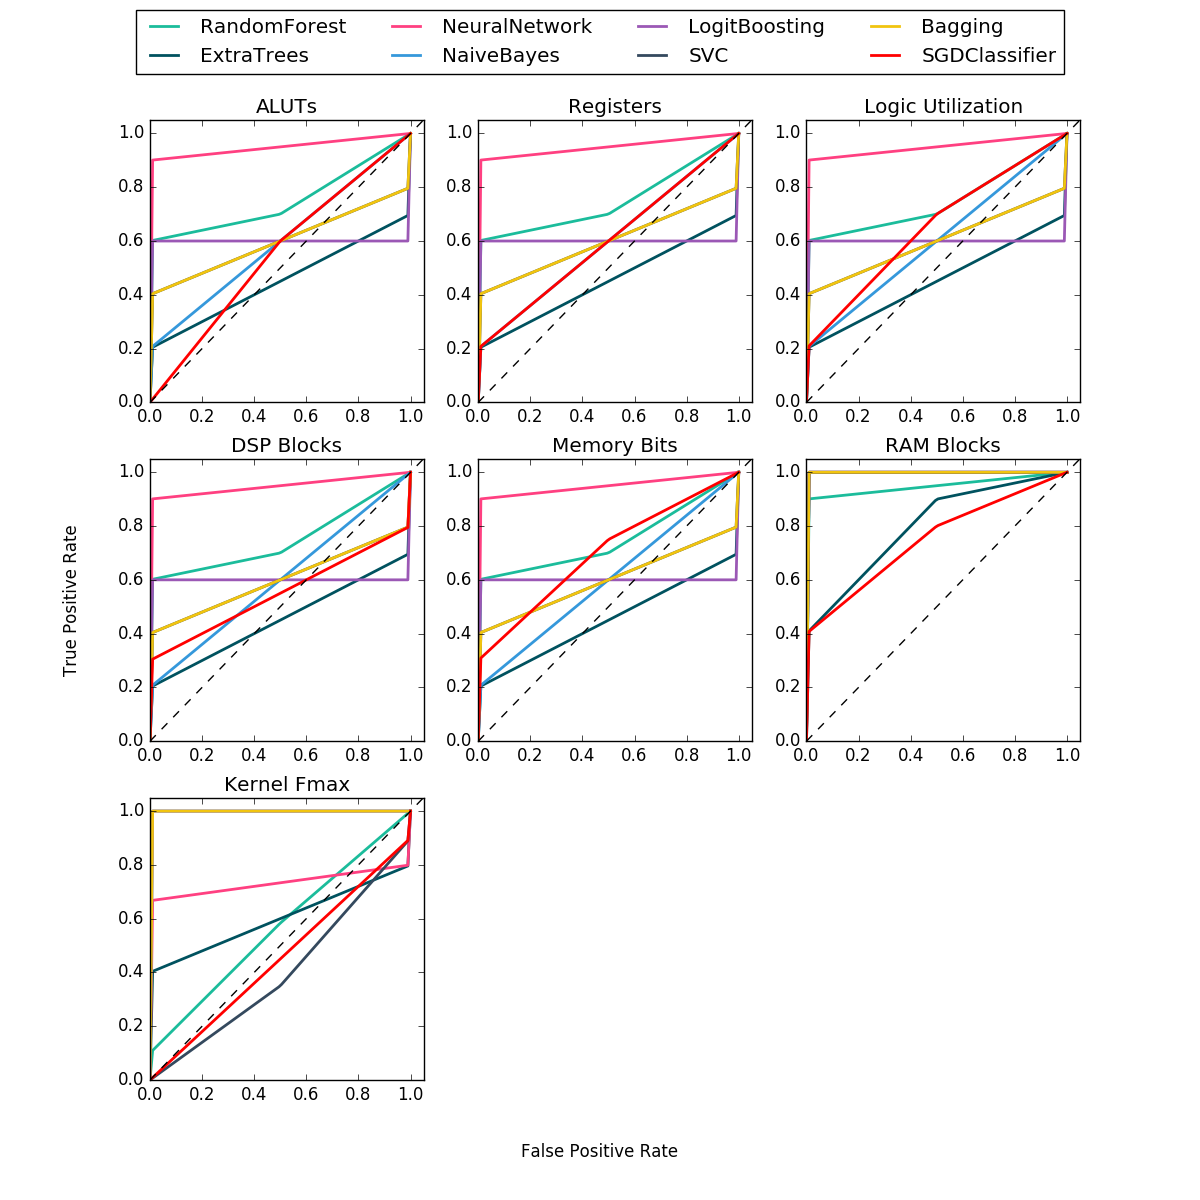
\includegraphics[scale=0.4]{dfmul_roc_curve.png}
\caption{ROC curve for dfmul benchmarks}
\label{figure:dfmul_roc_curve}
\end{figure}

\begin{figure}[h!]
\centering
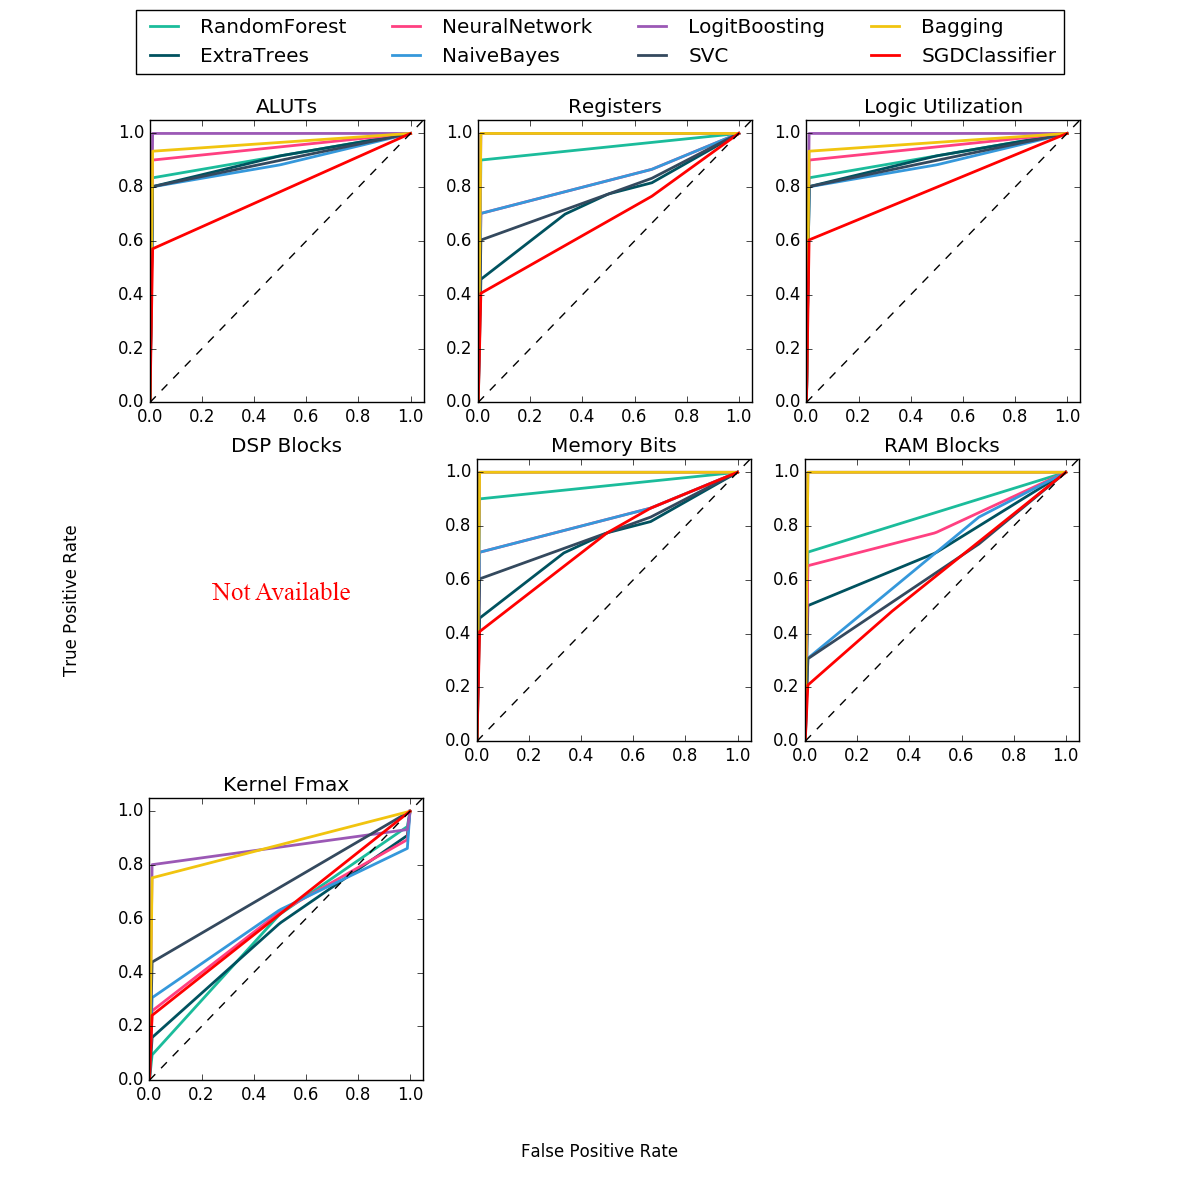
\includegraphics[scale=0.4]{dfadd_roc_curve.png}
\caption{ROC curve for dfadd benchmarks}
\label{figure:dfadd_roc_curve}
\end{figure}
